\section{Handling Other Practical Issues in Linear Regression}

So far in this chapter, we have learned:
\begin{itemize}
	\item How to implement a linear regression model using multiple practical approaches.
	\item How to measure and evaluate model efficiency using goodness-of-fit parameters and diagnostics.
\end{itemize}

However, additional empirical challenges frequently arise when working with diverse datasets in real-world scenarios. Let us examine these practical issues one by one. We will use a simulated dataset (\texttt{EcomExpense.csv}) to illustrate these challenges. Let us import the dataset and inspect its initial rows:

\begin{lstlisting}[language=Python]
import pandas as pd
df = pd.read_csv('./dataBases/EcomExpense.csv')
print(df.head())
\end{lstlisting}

Executing this script should produce the following output table:

\begin{lstlisting}[language=Python]
  Transaction ID  Age  Items  Monthly Income  Transaction Time  Record  \
0         TXN001   42     10            7313        627.668127       5   
1         TXN002   24      8           17747        126.904567       3   
2         TXN003   47     11           22845        873.469701       2   
3         TXN004   50     11           18552        380.219428       7   
4         TXN005   60      2           14439        403.374223       2   

   Gender City Tier  Total Spend  
0  Female    Tier 1  4198.385084  
1  Female    Tier 2  4134.976648  
2    Male    Tier 2  5166.614455  
3  Female    Tier 1  7784.447676  
4  Female    Tier 2  3254.160485  
\end{lstlisting}

The output above captures simulated transaction records from an e-commerce website. Specifically, it tracks user demographic profile characteristics and browsing behaviors associated with individual purchase transactions.

A brief description of the dataset variables is as follows:
\begin{itemize}
	\item \texttt{Transaction ID}: Unique alphanumeric identifier for each purchase transaction.
	\item \texttt{Age}: Customer's age in years.
	\item \texttt{Items}: Total number of merchandise items added to the shopping cart and purchased.
	\item \texttt{Monthly Income}: Customer's monthly disposable income in dollars.
	\item \texttt{Transaction Time}: Total time in seconds spent actively browsing the website during the session.
	\item \texttt{Record}: Historical count indicating how many previous purchase transactions the customer has completed.
	\item \texttt{Gender}: Customer's biological or reported gender classification (\texttt{Male} / \texttt{Female}).
	\item \texttt{City Tier}: Urban classification tier of the customer's residence (\texttt{Tier 1}, \texttt{Tier 2}, \texttt{Tier 3}).
	\item \texttt{Total Spend}: Total monetary expenditure recorded for the current transaction in dollars.
\end{itemize}

The primary output response variable is \texttt{Total Spend}. The remaining attributes serve as potential explanatory predictors, and our initial modeling hypothesis is that total expenditure is linearly related to these predictor attributes.

\subsection{Handling Categorical Variables}

Until now, we have assumed that our explanatory predictors must be strictly continuous or quantitative variables. However, real-world analytical problems frequently involve datasets that \emph{contain categorical or qualitative variables}. Furthermore, these qualitative attributes often exert a profound and statistically significant influence on the target response. Therefore, a critical practical question arises: \emph{How do we properly encode and process qualitative attributes so that they can be incorporated into a quantitative regression specification?}

We cannot simply assign numerical codes directly to qualitative categories (such as $0, 1, 2, \dots$) and insert those raw integers into our linear regression model. Doing so would artificially impose numerical weighting and false metric intervals between qualitative categories based purely on arbitrary coding assignments.

Direct integer coding of nominal categories almost inevitably leads to biased, erroneous regression slopes, because the estimated parameters will fluctuate wildly whenever the arbitrary integer mapping assigned to those categories is changed.

In the e-commerce data frame just imported, \texttt{Gender} and \texttt{City Tier} represent qualitative categorical attributes.

To incorporate qualitative categorical attributes accurately into a regression architecture, we construct indicator variables, commonly referred to as **dummy variables**.

A linear regression model containing categorical predictors takes the general form:
\begin{align}
	Y_{\texttt{model}} = \a + \sum \beta_{i} X_{i}
\end{align}
where certain $X_{i}$ terms represent qualitative dummy predictors. Let $X_{g}$ denote one such binary indicator attribute.

In our e-commerce example, we can encode customer gender using a binary indicator variable defined as:
\begin{align}
	X_{g} =
	\begin{cases}
		1 & \text{if customer is Male} \\
		0 & \text{if customer is Female}
	\end{cases}
\end{align}

When a qualitative attribute possesses more than two distinct categories ($n > 2$), multiple dummy variables must be generated to capture all possible states without ambiguity. Specifically, if a categorical variable has three distinct levels, two dummy variables must be defined relative to a baseline reference category.

For example, the variable \texttt{City Tier} contains three distinct urban levels across our dataset.

To encode these three categories without introducing collinear redundancy, we define two binary indicator variables as follows:
\begin{align}
	X_{t1} =
	\begin{cases}
		1 & \text{if } \texttt{City Tier} = \text{Tier 1} \\
		0 & \text{if } \texttt{City Tier} \neq \text{Tier 1}
	\end{cases}
\end{align}
\begin{align}
	X_{t2} =
	\begin{cases}
		1 & \text{if } \texttt{City Tier} = \text{Tier 2} \\
		0 & \text{if } \texttt{City Tier} \neq \text{Tier 2}
	\end{cases}
\end{align}

Under this encoding scheme, our predictive regression model evaluates across the three urban categories according to the following system of equations:
\begin{align}
	Y =
	\begin{cases}
		\a + \beta_{1}X_{1} + \dots + \beta_{t1}(1) + \beta_{t2}(0) + \dots + \beta_{n}X_{n} & \text{if } \texttt{City Tier} = \text{Tier 1} \\
		\a + \beta_{1}X_{1} + \dots + \beta_{t1}(0) + \beta_{t2}(1) + \dots + \beta_{n}X_{n} & \text{if } \texttt{City Tier} = \text{Tier 2} \\
		\a + \beta_{1}X_{1} + \dots + \beta_{t1}(0) + \beta_{t2}(0) + \dots + \beta_{n}X_{n} & \text{if } \texttt{City Tier} = \text{Tier 3}
	\end{cases}
\end{align}

Notice that we do not need to generate a third dummy variable ($X_{t3}$) explicitly. This structural property stems directly from the mutually exclusive and exhaustive nature of categorical indicators.

If a customer resides neither in Tier 1 ($X_{t1}=0$) nor in Tier 2 ($X_{t2}=0$), then logically and necessarily that customer resides in Tier 3. Therefore, an explicit dummy variable is omitted for one reference category to prevent exact linear dependence across columns (known as the **dummy variable trap**).

\begin{observacion}
	As a general structural rule, when encoding a qualitative categorical variable containing $n$ distinct nominal levels into a linear regression model with an intercept, one should construct exactly $(n - 1)$ binary dummy variables.
\end{observacion}

However, for didactic demonstration purposes and when using specific regularized or non-intercept formulations, one may sometimes construct binary indicator columns for every category explicitly.

Let us now construct the binary dummy variables for our categorical attributes and append them directly to our working data frame using Python:

\begin{lstlisting}[language=Python]
dummy_gender = pd.get_dummies(df['Gender'], prefix='Sex')
dummy_city_tier = pd.get_dummies(df['City Tier'], prefix='City')
\end{lstlisting}

Let us inspect the resulting binary matrices to confirm that they satisfy our logical conditions. The output structure for \texttt{dummy\_city\_tier} is:

\begin{lstlisting}[language=Python]
   City_Tier 1  City_Tier 2  City_Tier 3
0            1            0            0
1            0            1            0
2            0            1            0
3            1            0            0
4            0            1            0
\end{lstlisting}

Similarly, the structure of \texttt{dummy\_gender} takes the following form:
\begin{lstlisting}[language=Python]
   Sex_Female  Sex_Male
0           1         0
1           1         0
2           0         1
3           1         0
4           1         0
\end{lstlisting}

We now have these dummy variable data frames generated, but they are not yet merged into our primary working data frame (\texttt{df}). Let us concatenate these new indicator columns into our main data frame so that they can be utilized directly during regression fitting:

\begin{lstlisting}[language=Python]
df2 = pd.concat([df, dummy_gender, dummy_city_tier], axis=1)
print(df2.head())
\end{lstlisting}

This concatenation yields the expanded data frame structure:

\begin{lstlisting}[language=Python]
  Transaction ID  Age  Items  Monthly Income  Transaction Time  Record  \
0         TXN001   42     10            7313        627.668127       5   
1         TXN002   24      8           17747        126.904567       3   
2         TXN003   47     11           22845        873.469701       2   
3         TXN004   50     11           18552        380.219428       7   
4         TXN005   60      2           14439        403.374223       2   

   Gender City Tier  Total Spend  Sex_Female  Sex_Male  City_Tier 1  \
0  Female    Tier 1  4198.385084           1         0            1   
1  Female    Tier 2  4134.976648           1         0            0   
2    Male    Tier 2  5166.614455           0         1            0   
3  Female    Tier 1  7784.447676           1         0            1   
4  Female    Tier 2  3254.160485           1         0            0   

   City_Tier 2  City_Tier 3  
0            0            0  
1            1            0  
2            1            0  
3            0            0  
4            1            0  
\end{lstlisting}

Notice that five new indicator columns have been appended to the data frame: two binary dummy variables representing \texttt{Gender} (\texttt{Sex\_Female}, \texttt{Sex\_Male}) and three binary dummy variables representing \texttt{City Tier} (\texttt{City\_Tier 1}, \texttt{City\_Tier 2}, \texttt{City\_Tier 3}).

Inspecting these binary columns against the original categorical text columns confirms that \texttt{City\_Tier\_1} contains value $1$ whenever \texttt{City Tier} equals \texttt{Tier 1}, \texttt{City\_Tier\_2} contains value $1$ whenever \texttt{City Tier} equals \texttt{Tier 2}, and \texttt{City\_Tier\_3} contains value $1$ whenever \texttt{City Tier} equals \texttt{Tier 3}. All other dummy columns along that specific observation row correctly contain $0$. This matches our exact encoding requirements.

Let us now incorporate these newly created dummy predictors into a multiple linear regression model and evaluate the estimated regression coefficients.

For this dataset, assume a linear functional relationship between the target response variable \texttt{Total Spend} and our continuous predictors (\texttt{Monthly Income}, \texttt{Transaction Time}), alongside both sets of qualitative dummy variables:

\begin{lstlisting}[language=Python]
from sklearn.linear_model import LinearRegression

feature_cols = [
    'Monthly Income', 'Transaction Time',
    'City_Tier 1', 'City_Tier 2', 'City_Tier 3',
    'Sex_Female', 'Sex_Male'
]
X = df2[feature_cols]
Y = df2['Total Spend']

lm = LinearRegression()
lm.fit(X, Y)
\end{lstlisting}

We can extract the estimated model parameters using the following code block:
\begin{lstlisting}[language=Python]
print(lm.intercept_)
for _ in zip(feature_cols, lm.coef_):
    print(_)
\end{lstlisting}

Running this script outputs the estimated intercept and partial regression slopes:
\begin{lstlisting}[language=Python]
3655.72940769
('Monthly Income', 0.15297824609320512)
('Transaction Time', 0.12372608642619998)
('City_Tier 1', 119.66325160390086)
('City_Tier 2', -16.67901800799039)
('City_Tier 3', -102.9842335959104)
('Sex_Female', -94.157798830320132)
('Sex_Male', 94.157798830320118)
\end{lstlisting}

The sample coefficient of determination ($R^2$) for this multiple regression specification is obtained via:
\begin{lstlisting}[language=Python]
R2 = lm.score(X, Y)
print(R2)
## 0.194789205529
\end{lstlisting}

The resulting $R^2$ turns out to be only $0.19$, which indicates that our current specification accounts for only about $19\%$ of the variance in total expenditure. This low explanatory power likely occurs because we omitted other critical predictors that correlate strongly with total spending behavior.

We can improve model accuracy by incorporating additional informative variables or applying appropriate feature transformations.

For example, if we add the historical transaction count variable (\texttt{Record}) to our predictor matrix, the $R^2$ jumps dramatically from $0.19$ up to $0.91$ (we encourage you to test this addition independently). This dataset provides an excellent playground for exploring feature selection dynamics.

The fitted predictive equation incorporating our initial dummy variables can be written explicitly as:
\begin{align}
	\texttt{Total\_Spend} \approx & \, 3655.73 + 0.12 \times \texttt{Transaction Time} \nonumber \\
	& + 0.15 \times \texttt{Monthly Income} + 119.66 \times \texttt{City\_Tier 1} \nonumber \\
	& - 16.68 \times \texttt{City\_Tier 2} - 102.98 \times \texttt{City\_Tier 3} \nonumber \\
	& - 94.16 \times \texttt{Sex\_Female} + 94.16 \times \texttt{Sex\_Male}
\end{align}

The Residual Standard Error (\texttt{RSE}) for this fitted specification can be computed as follows:

\begin{lstlisting}[language=Python]
import numpy as np

df2['total_spend_pred'] = (
    3655.72940769
    + 0.12372608 * df2['Transaction Time']
    + 0.15297825 * df2['Monthly Income']
    + 119.66325160 * df2['City_Tier 1']
    - 16.67901801 * df2['City_Tier 2']
    - 102.98423360 * df2['City_Tier 3']
    - 94.15779883 * df2['Sex_Female']
    + 94.15779883 * df2['Sex_Male']
)

df2['SSD'] = (df2['Total Spend'] - df2['total_spend_pred']) ** 2
SSD = df2.sum()['SSD']
RSE = np.sqrt(SSD / (len(df2) - len(feature_cols) - 1))
salesmean = np.mean(df2['Total Spend'])
error = RSE / salesmean

print(RSE, salesmean, error)
## 2518.85203887 6163.176415976714 0.408693808008
\end{lstlisting}

The resulting \texttt{RSE} is approximately $2518.85$ over an average transaction spend of $6163.18$, which corresponds to a relative predictive error of roughly $40.87\%$.

Across different combinations of customer gender and city classification tiers, our general multi-dummy model simplifies structurally into distinct parallel response equations for each specific demographic segment:

\begin{center}
	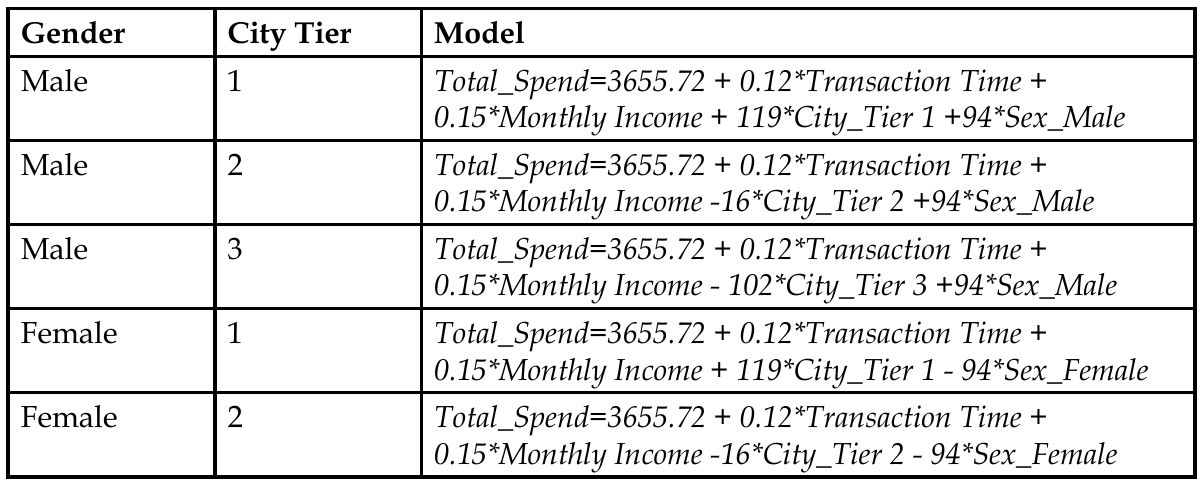
\includegraphics[width=10cm,keepaspectratio=true]{./images/dummies.png}
	\% dummies.png: 0x0 pixel, 300dpi, 0.00x0.00 cm, bb=
\end{center}

\subsection{Transforming Predictor Variables to Capture Non-Linear Relationships}

Frequently, the quantitative target variable does not maintain a straight linear relationship with one or more continuous explanatory variables; instead, the underlying physical or economic phenomenon exhibits a **non-linear functional relationship**.

Such non-linear patterns can range from simple curvilinear trends (such as quadratic, polynomial, exponential, or logarithmic curves) to complex higher-order polynomial surfaces. Under these conditions, applying mathematical variable transformations provides an effective and powerful mechanism to linearize the relationship so that classical OLS regression architectures can still be employed.

The following step-by-step diagnostic guideline outlines how to identify and model non-linear predictor relationships effectively:
\begin{enumerate}
	\item Plot a two-dimensional scatter plot comparing the response variable against each continuous predictor variable individually. (In multivariate settings, you can construct a comprehensive scatter plot matrix, similar in spirit to a correlation heatmap matrix).
	\item If the scattered points cluster along an approximately straight diagonal trend line, the predictor is linearly related to the response variable and can be entered into the regression specification without modification.
	\item If the scatter plot reveals a distinct, systematic curvature or non-linear trajectory (such as a parabolic arc, asymptotic curve, or logarithmic saturation), we apply an appropriate mathematical transformation (e.g., squaring, taking square roots, or taking logarithms) to that predictor before fitting the linear regression model.
\end{enumerate}

Let us demonstrate this transformation process using an empirical automotive dataset (\texttt{Auto.csv}). This dataset contains technical specifications—including fuel efficiency in miles per gallon (\texttt{mpg}), engine power (\texttt{horsepower}), vehicle weight, and displacement—for numerous historical automobile models. Here, \texttt{mpg} serves as our primary response variable, which is known to depend strongly on engine power (\texttt{horsepower}).

\begin{lstlisting}[language=Python]
import pandas as pd
data = pd.read_csv('./dataBases/Auto.csv')
print(data.head())
\end{lstlisting}

Executing this script displays the initial vehicle records:

\begin{lstlisting}[language=Python]
    mpg  cylinders  displacement  horsepower  weight  acceleration  \
0  18.0          8         307.0       130.0    3504          12.0   
1  15.0          8         350.0       165.0    3693          11.5   
2  18.0          8         318.0       150.0    3436          11.0   
3  16.0          8         304.0       150.0    3433          12.0   
4  17.0          8         302.0       140.0    3449          10.5   

   model year  origin                   car name  
0          70       1  chevrolet chevelle malibu  
1          70       1          buick skylark 320  
2          70       1         plymouth satellite  
3          70       1              amc rebel sst  
4          70       1                ford torino  
\end{lstlisting}

The dataset contains $406$ rows across $9$ columns. Notice that certain columns contain missing or non-available entries (\texttt{NA}), making it necessary to clean and impute or drop missing records before running regression models.

Let us now plot a scatter plot comparing \texttt{horsepower} against \texttt{mpg} to diagnose whether the functional relationship follows a straight line or exhibits significant non-linear curvature:

\begin{lstlisting}[language=Python]
import matplotlib.pyplot as plt

data['mpg'] = pd.to_numeric(data['mpg'], errors='coerce')
data['horsepower'] = pd.to_numeric(data['horsepower'], errors='coerce')
data_clean = data.dropna(subset=['mpg', 'horsepower'])

plt.figure(figsize=(8, 6))
plt.plot(data_clean['horsepower'], data_clean['mpg'], 'ro', alpha=0.6)
plt.xlabel('Horsepower')
plt.ylabel('MPG (Miles Per Gallon)')
plt.title('Scatter Plot: Horsepower vs. MPG')
plt.show()
\end{lstlisting}

\begin{figure}
	\centering
	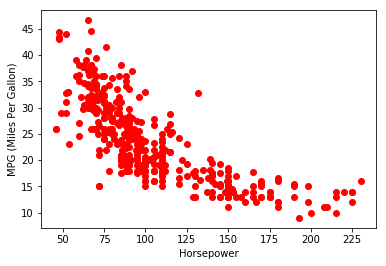
\includegraphics[width=10cm,keepaspectratio=true]{./images/hpVsMpg.png}
	\% hpVsMpg.png: 0x0 pixel, 300dpi, 0.00x0.00 cm, bb=
	\caption{\texttt{Horsepower vs. MPG}}
	\label{fig:4.12.1}
\end{figure}

Although we might initially hypothesize a simple linear relationship:
\begin{align}
	\texttt{mpg} = c_{0} + c_{1} \times \texttt{hp}
\end{align}
visual inspection of the scatter plot reveals unmistakable downward curvature. The points clearly follow a curved, parabolic trajectory much better described by a **quadratic polynomial model**:
\begin{align}
	\texttt{mpg} = c_{0} + c_{1} \times \texttt{hp} + c_{2} \times \texttt{hp}^{2}
\end{align}

Let us first fit a straight linear regression line between \texttt{horsepower} and \texttt{mpg} to establish a baseline comparison. We impute missing values using sample column means before fitting the model:

\begin{lstlisting}[language=Python]
import numpy as np
from sklearn.linear_model import LinearRegression

X = data['horsepower'].fillna(data['horsepower'].mean())
Y = data['mpg'].fillna(data['mpg'].mean())

lm = LinearRegression()
lm.fit(X.values[:, np.newaxis], Y)
\end{lstlisting}

Notice that \texttt{scikit-learn}'s regression estimators require predictor matrix \texttt{X} to be formatted strictly as a two-dimensional array. Using \texttt{np.newaxis} (or \texttt{.values.reshape(-1, 1)}) explicitly inserts the required column dimension.

We can plot the fitted straight regression line over the scatter plot using the following script:

\begin{lstlisting}[language=Python]
import matplotlib.pyplot as plt

plt.figure(figsize=(8, 6))
plt.plot(data['horsepower'], data['mpg'], 'ro', alpha=0.6)
plt.plot(X, lm.predict(X.values[:, np.newaxis]), color='blue', linewidth=2)
plt.xlabel('Horsepower')
plt.ylabel('MPG')
plt.title('Linear Fit: Horsepower vs. MPG')
plt.show()
\end{lstlisting}

\begin{center}
	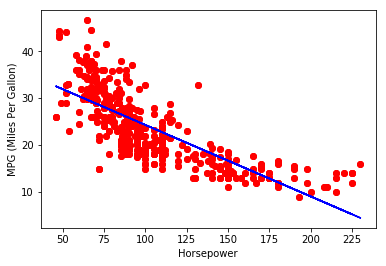
\includegraphics[width=10cm,keepaspectratio=true]{./images/hpLR.png}
	\% hpLR.png: 0x0 pixel, 300dpi, 0.00x0.00 cm, bb=
\end{center}

We evaluate the numerical performance metrics of this linear baseline model:
\begin{lstlisting}[language=Python]
R2 = lm.score(X.values[:, np.newaxis], Y)
print("Linear R2:", R2)
## 0.574653340645

RSEd = (Y - lm.predict(X.values[:, np.newaxis])) ** 2
RSE = np.sqrt(np.sum(RSEd) / (len(Y) - 2))
ymean = np.mean(Y)
error = RSE / ymean

print("Linear RSE:", RSE, "Relative Error:", error)
## 5.1496254787 0.21899719414
\end{lstlisting}

Here, we call the \texttt{.predict()} method directly to generate model predictions across all data rows.

The Residual Standard Error (\texttt{RSE}) for our straight linear specification turns out to be roughly $5.15$. Over a mean fuel efficiency of $23.51\text{ mpg}$, this corresponds to an average predictive error of approximately $21.9\%$ ($22\%$).

To capture the observed curvature accurately, we fit a second-degree polynomial (quadratic) specification using \texttt{scikit-learn}'s \texttt{PolynomialFeatures} preprocessor class. This transformation automatically generates both linear (\texttt{hp}) and squared ($\texttt{hp}^2$) columns:

\begin{lstlisting}[language=Python]
from sklearn.preprocessing import PolynomialFeatures
from sklearn import linear_model

X = data['horsepower'].fillna(data['horsepower'].mean())
Y = data['mpg'].fillna(data['mpg'].mean())

poly = PolynomialFeatures(degree=2)
X_poly = poly.fit_transform(X.values[:, np.newaxis])

clf = linear_model.LinearRegression()
clf.fit(X_poly, Y)

print("Intercept:", clf.intercept_)
## 55.0261924471
print("Coefficients:", clf.coef_)
## [ 0.         -0.43404318  0.00112615]
\end{lstlisting}

The estimated quadratic regression equation can be written explicitly as:
\begin{align}
	\texttt{mpg} = 55.03 - 0.434 \times \texttt{hp} + 0.00113 \times \texttt{hp}^{2}
\end{align}

We can visualize how this quadratic polynomial curve fits the underlying automobile data scatter much more smoothly and accurately than the straight line:

\begin{lstlisting}[language=Python]
plt.figure(figsize=(8, 6))
plt.plot(data['horsepower'], data['mpg'], 'ro', alpha=0.6, label='Observed Data')

# Sort X for smooth curve plotting
sort_idx = np.argsort(X.values)
plt.plot(X.values[sort_idx], clf.predict(X_poly[sort_idx]), color='blue', linewidth=2.5, label='Quadratic Fit')

plt.xlabel('Horsepower')
plt.ylabel('MPG')
plt.title('Quadratic Fit: Horsepower vs. MPG')
plt.legend()
plt.show()
\end{lstlisting}

\begin{center}
	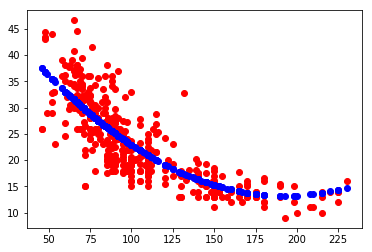
\includegraphics[width=10cm,keepaspectratio=true]{./images/hpNLR.png}
	\% hpNLR.png: 0x0 pixel, 300dpi, 0.00x0.00 cm, bb=
\end{center}
